\section{Проектирование синхронного фреймворка}

Один из основных подходов, используемых при разработке платформы – это максимальная гибкость и расширяемость. В платформе используется абстракция – механизм, представляющая собой и на деле некий механизм, ответственный за определенную задачу синхронизации внутри платформы. При желании, разработчик, использующий платформу может для разных задач использовать готовые механизмы, но если считает, что они ему не подходят, то может добавлять свои механизмы, расширяя функционал платформы. В дальнейшем все вызовы будут обработаны в одном потоке, что исключает гонку за данные.

Продемонстрировать гибкость платформы можно наглядно на следующем примере: в платформе есть механизм, ответственный за запуск и исполнение всех модулей в системе; есть несколько вариантов этого механизма – обычный линейный, многопоточный, многопоточный с использованием пула потоков. При использовании системы на различных процессорах – одноядерных или многоядерных имеет смысл использовать различные режимы исполнения соответственно, чтобы исключить затраты на лишнюю синхронизацию и обеспечить максимальную производительность. Так, например, нет смысла запускать многопоточный режим на старом одноядерном процессоре, и в ту же очередь нет смысла не использовать возможность распараллеливания на многоядерных процессорах. Гибкость и расширяемость описываемой платформы позволяет подстроить ее под необходимую среду, в которой ей придется работать.

В данной реализации под механизмами будет подразумеваться класс-обертка вокруг потоконебезопасного класса, которая инкапсулирует все вызовы к данному классу в функциональный объект и помещает его в потокобезопасную очередь. Использование механизма отложенных синхронизаций позволяет избавиться от проблем зацикливания при ситуации, например, когда какой-нибудь модуль отправляет сообщения сам себе. Также, позволяет с легкостью подобрать нужную реализацию очереди под конкретную ситуацию. В асинхронной версии библиотеки структура механизма отличается от описанной в данном разделе.

Ниже, на рис. \ref{im:2_2_1_sync}, представлена схема синхронного прототипа ядра системы. Данная диаграмма классов включает только основной набор классов, которые демонстрируют механику взаимодействия между отдельными компонентами системы:

\begin{figure}[h]
    \centering{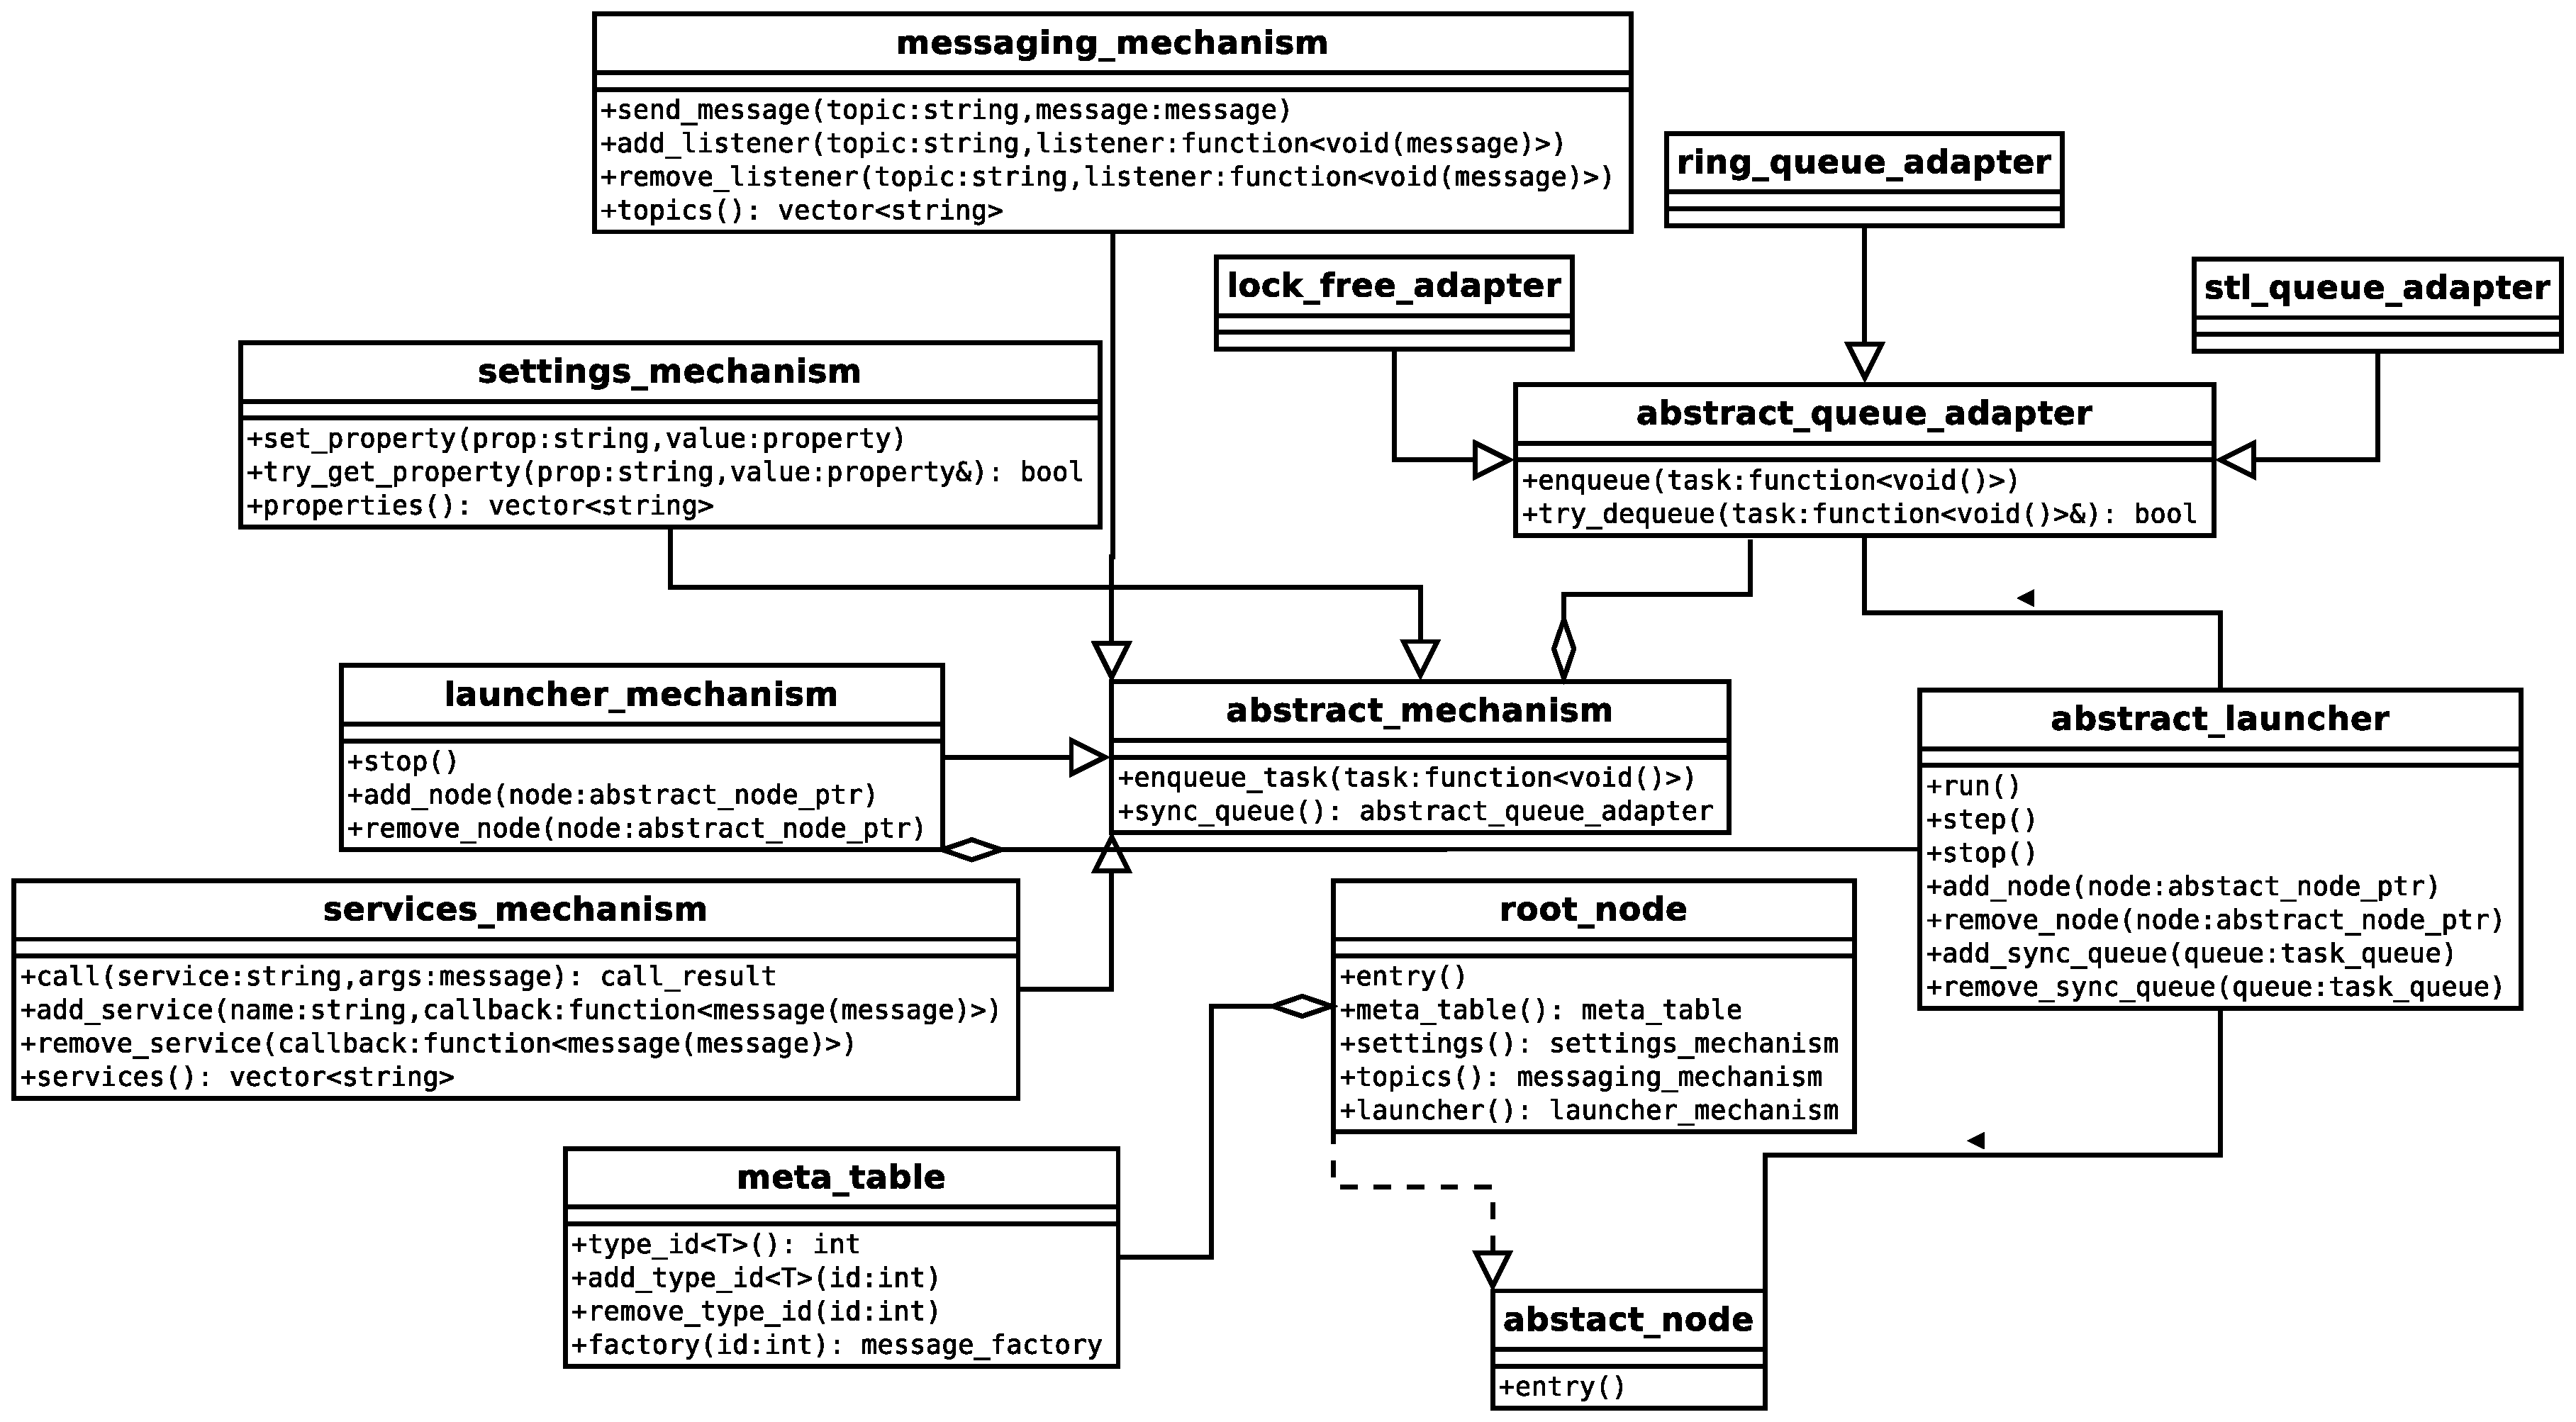
\includegraphics[width=1\linewidth]{2_2_1_sync}}
    \caption{Диаграмма классов синхронной версии фреймворка}
    \label{im:2_2_1_sync}
\end{figure}

\textit{abstract\_launcher} --- интерфейс исполняющего класса. Реализация данного класса должна хранить указатели на модули и очереди синхронизаций и обеспечивать требуемый порядок исполнения, например, последовательно в одном потоке или с использованием пула потоков.

\textit{abstract\_queue\_adapter} --- интерфейс компонента, необходимого для обеспечения отложенной синхронизации. Он передает все задачи по синхронизации на определенные очереди. Адаптер предоставляет единый интерфейс для добавления и получения элементов из очереди. Его возможные реализации:

\textit{stl\_queue\_adapter} --- компонент, необходимый для работы с очередью из стандартной библиотеки c++ STL. В данном классе не используются блокировки для повышения производительности на одноядерных системах

\textit{lock\_free\_adapter} --- компонент, необходимый для работы с lock-free(без использования мъютексов) очередью. В проекте используется реализация очереди Камерона Десрочерза (Cameron Desrochers).

\textit{ring\_queue\_adapter} --- компонент, необходимый для работы с  циклической очередью фиксированного размера.

\textit{abstract\_node} --- интерфейс, позволяющий создавать независимые компоненты системы --- модули, каждый из которых может быть ответственнен за свой конкретный функционал. Модули не знают о существовании других модулей, то есть, они на самом деле, полностью независимы друг от друга. Из взаимодействие и исполнение обеспечено ядром системы. Такой подход к созданию этой абстракции также позволяет переиспользовать разработанные на ее основе модули при различных конфигурациях описываемой робототехнической платформы, а так же позволяет исполнять каждый модуль в отдельном потоке без дополнительных затрат процессорного времени на синхронизацию. 

\textit{abstract\_mechanism} --- абстрактный класс для компонентов системы, обеспечивающих какой-либо потокобезопасный вид взаимодействия между модулями и с ядром системы. Класс содержит потокобезопасную очередь функциональных объектов, куда помещаются все вызовы к базовому классу. Для функционирования механизма Указатель на очередь должен быть зарегистрирован в экземпляре класса abstract\_launcher.

\textit{launcher\_mechanism} --- компонет, реализующий интерфейс abstract\_mechanism, обеспечивающий взаимодействий с конкретной реализацией abstarct\_launcher, позволяет добавлять и удалять модули, запускать и останавливать систему.

\textit{messaging\_mechanism} --- компонет, реализующий интерфейс abstract\_mechanism, обеспечивающий возможность коммуникации и обмена данными между модулями путем отправки сообщений. Данный механизм реализован с использованием паттерна <<издатель-подписчик>>. Экземпляр <<слушателя>> добавляется в список к именованному <<топику>>, куда в дальнейшем любой модуль может отправлять отправлять сообщения. Данный механизм реализован по аналогии с системой рассылки сообщений в ROS.

\textit{services\_mechanism} --- компонет, реализующий интерфейс abstract\_mechanism, обеспечивающий возможность запуска требуемых методов по их имени. Вызовы происходят в неблокирующем режиме, поэтому система позволяет отправить несколько запросов до получения ответа. Аргументы метода передаются в структуре сообщения. Результат выполнения будет записан в объект результата после выполнения функции. 

\textit{meta\_table} --- класс, который содержит информацию для идентификации сообщений. В данной реализации использовалась библиотека google protocol buffers. Поскольку в данной библиотеке используется не тривиальный алгоритм сериализации и десериализации, сообщения внутри системы передаются в <<сыром>> виде для уменьшения дополнительных нагрузок на систему. При регистрации нового типа сообщений так же создается экземпляр фабрики для сообщений, который позволяет при получении сериализированных данных верифицировать их и создать экземпляр сообщения.

Следует так же уделить внимание классу сообщений \textit{message}. В данной реализации, как было сказанно ранее, используется библиотке google protocol buffers для генерации сериализируемых сообщений. Сериализация необходима, например, для передачи сообщения через сетевой протокол. Сообщения хранятся и передаются внутри системы через умные указатели (\textit{std::shared\_pointer}) на экземпляр структуры, которая хранит данные. Данный прием позволяет передавать сообщения внутри системы без дополнительных затрат на копирование данных, а так же автоматически освобождать занятые ресурсы памяти, что дает существенный прирост в производительности всей системы при рассылке сообщений нескольким <<слушателям>>.

По умолчанию в системе реализован класс \textit{abstract\_launcher}, который поочередно запускает обработку модулей и стадию синхронизации. Такой порядок исполенения позволяет исключить гонку за данные при многопоточном исполнении, а следовательно упростить структуру модулей в случае, если модуль не создает собственного потока исполнения. На рис. \ref{im:2_2_2_sequence_diag} представленна диаграмма последовательностей, в которой изображен сценарий коммуникации модулей с ядром системы (механизмами синхронизации).

\begin{figure}[h]
    \centering{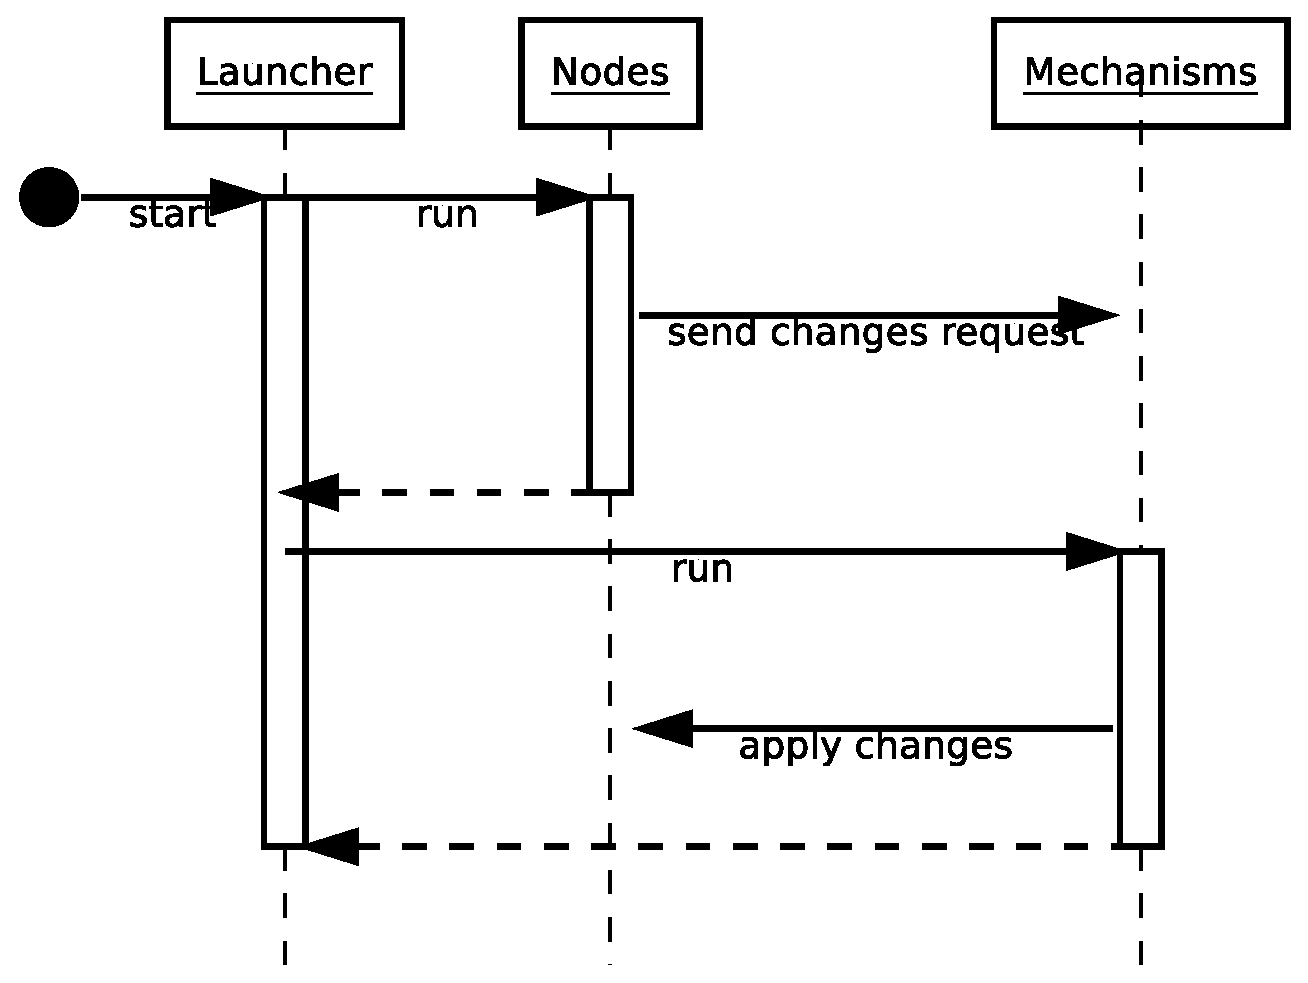
\includegraphics[width=0.7\linewidth]{2_2_2_sequence_diag}}
    \caption{Принцип работы класса \textit{abstract\_launcher}}
    \label{im:2_2_2_sequence_diag}
\end{figure}

Реализация механизмов синхронизации является ключевым звеном в разработке архитектуры данного фреймворка. Предполагается, что система работает в рамках одного адресного пространства и отдельные компоненты могут исполняться в отдельных потоках. Поскольку механизмы являются средством взаимодействия между модулями так же предполагается, что количество обращений к данным классам достаточно высоко и поэтому блокирующий вызов может существенно понизить отклик всей системы.

\begin{figure}[h]
    \centering{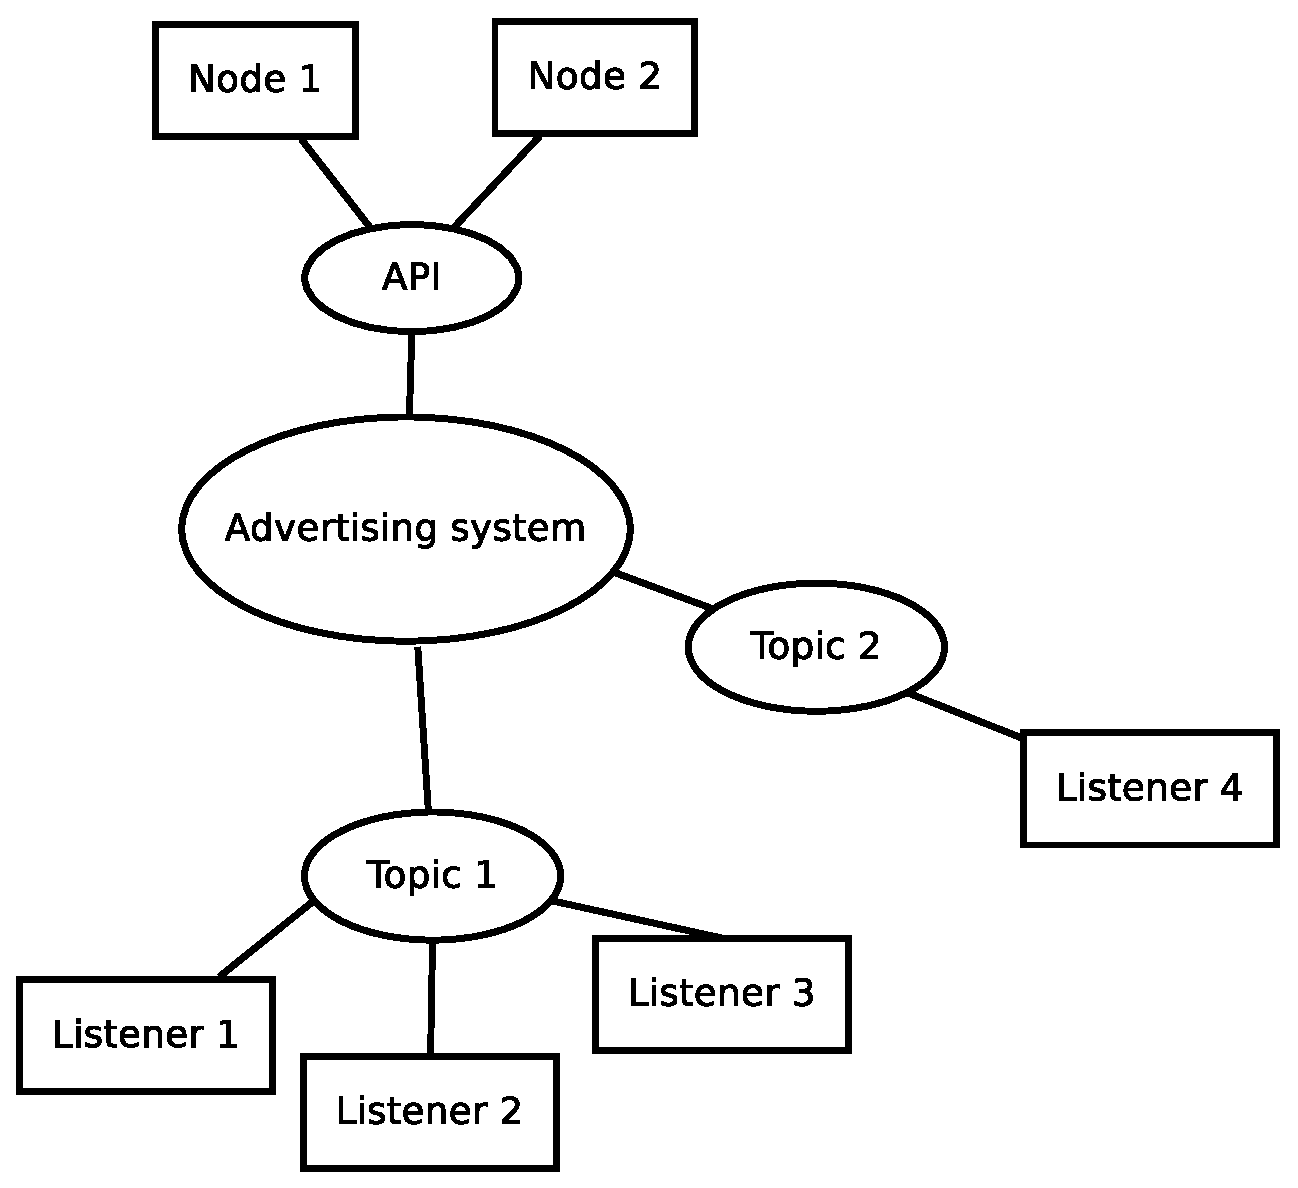
\includegraphics[width=0.7\linewidth]{2_2_3_topic}}
    \caption{Система рассылки сообщений}
    \label{im:2_2_3_topic}
\end{figure}

На рис. \ref{im:2_2_3_topic} схемматически изображен граф системы рассылки сообщений с двумя модулями, двумя топиками и четырьмя слушателями. На данном графике <<механизм>> выступает в роли API доступа к системе рассылки. Ребра графа показывают наличие возможности прямого вызова между компонентами системы круглые вершины обозначают компонент ядра системы, а прямоугольные - компоненты, реализованные пользователем.

Интерфейс системы рассылки сообщений включает в себя четыре функции: отправить сообщение в топик, получить список топиков, добавить слушателя сообщений в топик и удалить слушателя из топика. Топик может существовать только если у него есть хотя бы один подписчик - это требуется для освобождения памяти при удалении подписчиков.

Далее будут расмотренны различные варианты взаимодействия модулей с механизмом синхронизации на примере данной структуры в ситуации, когда модули обрабатываются параллельно.




